\documentclass{article}

\usepackage{gensymb}
\usepackage{enumitem}
\usepackage{amssymb}
\usepackage{wrapfig}
\usepackage{subfigure}
\usepackage{braket}
\usepackage{amsmath}
\usepackage{graphicx}
\usepackage{mathtools}
\usepackage[letterpaper, margin=1in]{geometry}
\setlength{\parindent}{0cm}

\title{Update on H Elastic Data Analysis}
\author{Tritium $(e,e'p)$ Experiment\\Efrain Segarra}
\begin{document}

\maketitle

The idea of this analysis is to understand corrections to our measured quantities by looking in the overconstrained kinematical setting, elastic e-p scattering. The goal of this analysis is to produce a shifting matrix for kinematic variables to aid the analysis of tritium/helium-3 data.\\

I performed this optimization for mid kinematics $(e,e'p)$ on the hydrogen-target data. I will proceed next to do the analysis for the fast kinematics on $(e,e'd)$ on the deuteron-target runs.

%%%%%%%%%%%%%%%%%%%%%%%%%%%%%%%%%%%%%%%%%%%%%%%%%%%%%%%%%%%%%%%%%%%%%%%%%%%%%%%%%%%%%%%%%
\section*{Most Recent Updates}
\begin{itemize}
\item{Finished preliminary adjustments for H data at mid kinematics. The method I used is not perfect, and in the future, I recommend fixing the central angles by use of optics data.}
\item{All ``expected" and measured distributions align, except for $P_\textrm{miss,y}$, which may be originating from the raster not being calibrated.} 
\item{The central angles had to be adjusted by 0.67mrad, 0.446mrad for LHRS and RHRS, respectively. The central momenta were adjusted by -0.268 MeV, -0.391 MeV for LHRS and RHRS, respectively. Of course the angular correction was the largest effect, and the momenta shift was small.}
\item{The method for optimizing the central angles and momenta was not perfect, and is described below. It was a first crack at an online calibration.}
\item{Changes to skimmer: implemented HALLA\_p variable, updated central angles based on surveys, and central angles/momenta for mid kinematics based on this optimization.}
\end{itemize}

%%%%%%%%%%%%%%%%%%%%%%%%%%%%%%%%%%%%%%%%%%%%%%%%%%%%%%%%%%%%%%%%%%%%%%%%%%%%%%%%%%%%%%%%%
\section*{Next Steps}
I will look at fast kinematics and apply optimization procedure again.

%%%%%%%%%%%%%%%%%%%%%%%%%%%%%%%%%%%%%%%%%%%%%%%%%%%%%%%%%%%%%%%%%%%%%%%%%%%%%%%%%%%%%%%%%
\section*{Assumptions Made}
First some brief definitions I'll use:
\begin{equation*}
	\begin{gathered}
		p_1^\mu \equiv (E_1,\vec{p}_1)	\textrm{     Electron beam}	\\
		p_2^\mu \equiv (m_p,\vec{0} )	\textrm{     Proton at rest}	\\
		p_3^\mu \equiv (E_3,\vec{p}_3)	\textrm{     Scattered electron}	\\
		p_4^\mu \equiv (E_4,\vec{p}_4)		\textrm{     Scattered proton}
	\end{gathered}
\end{equation*}

Since we are analyzing H data, we are overconstained in what we measure. By just looking at the scattering angles of $\theta_3,\theta_4$, we can determine (1) the beam energy, $E_1$, the scattered electron energy/momentum, $E_3=|\vec{p}_3|$, and (3) the scattered proton energy/momentum, $\vec{p}_4$.\\		

To do so, the first two equations I rederived last night, but originate from a CLAS Collaboration paper by D. Adikaram, et al., ``Towards a resolution of the proton form factor problem: new electron and positron scattering data". The third equation is just conservation of energy-momentum.\\
\begin{equation*}
	\begin{gathered}
		E_1 = m_p ( \cot{\frac{\theta_3}{2}} \cot{\theta_4} - 1 )	\\
		|\vec{p}_3| = E_3 = \frac{ m_p E_1 }{ m_p + E_1 (1-\cos{\theta_3} )}	\\
		|\vec{p}_4| = \sqrt{(E_1 + m_p - E_3)^2 - m_p^2}
	\end{gathered}
\end{equation*}

%%%%%%%%%%%%%%%%%%%%%%%%%%%%%%%%%%%%%%%%%%%%%%%%%%%%%%%%%%%%%%%%%%%%%%%%%%%%%%%%%%%%%%%%%
\section*{Cuts Applied}
The cuts I apply are used for all data sets, except of course I don`t include $\theta_{nq}$ cut:
\begin{itemize}
\item{$L_{E/P} <  0.5 $}
\item{$|L_z - R_z - 0.0037| < 0.018$}
\item{$|L_z| < 0.09 $}
\item{$|R_\delta| < 0.045 $}
\item{$|L_\delta| < 0.045 $}
\item{$ \left( R_{y\textrm{tar}} + \frac{1.5 R_{y'\textrm{tar}}}{0.08} \right)^2 + \left( \frac{1.5 R_{y'\textrm{tar}}}{0.08} \right)^2 < 1 $}
\item{$ \left( R_{x\textrm{tar}} + \frac{1.5 R_{x'\textrm{tar}}}{0.08} \right)^2 + \left( \frac{1.5 R_{x'\textrm{tar}}}{0.08} \right)^2 < 1 $}
\end{itemize}

%%%%%%%%%%%%%%%%%%%%%%%%%%%%%%%%%%%%%%%%%%%%%%%%%%%%%%%%%%%%%%%%%%%%%%%%%%%%%%%%%%%%%%%%%
\section*{Pre-Optimized Central Values Used}
These are the pre-optimized central kinematic values.
\begin{itemize}
\item{$\theta_e = 17.8003\degree$}
\item{$p_e = 3.543$ GeV}
\item{$\theta_p = 48.8094\degree$}
\item{$p_p = 1.481$ GeV}
\end{itemize}

%%%%%%%%%%%%%%%%%%%%%%%%%%%%%%%%%%%%%%%%%%%%%%%%%%%%%%%%%%%%%%%%%%%%%%%%%%%%%%%%%%%%%%%%%
\section*{Optimization Procedure}
Here I will outline the procedure method I used to optimze the central angles and momenta of the LHRS and RHRS. This procedure is a bit of a toy-model, and should be better optimized by use of optics data to fix the angles permamently. The drawback to this method is that I am under-constrained, and guessing a ``most-likely" solution.\\

Details.. details..\\

%%%%%%%%%%%%%%%%%%%%%%%%%%%%%%%%%%%%%%%%%%%%%%%%%%%%%%%%%%%%%%%%%%%%%%%%%%%%%%%%%%%%%%%%%
\section*{Results}
First, these are the kinematical distributions that are stored in the skimmed root file (i.e. NOT variables re-calculated based on scattering angles).
\begin{center}
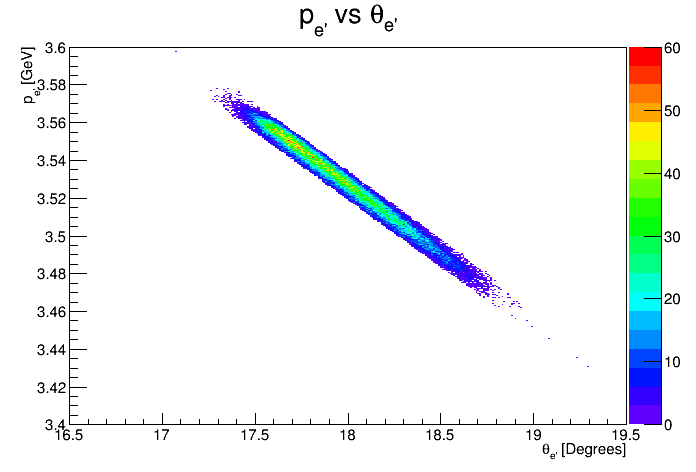
\includegraphics[width=15cm]{Pe_Te.png}\\
Scattered electron angle and momentum.
\end{center}

\begin{center}
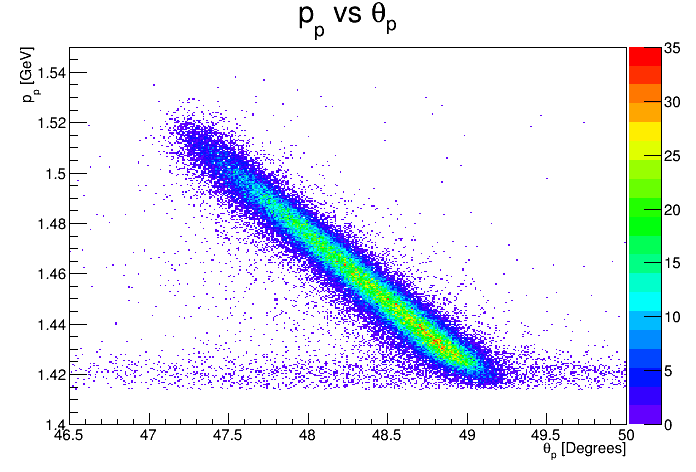
\includegraphics[width=15cm]{Pp_Tp.png}\\
Scattered proton angle and momentum.
\end{center}

\begin{center}
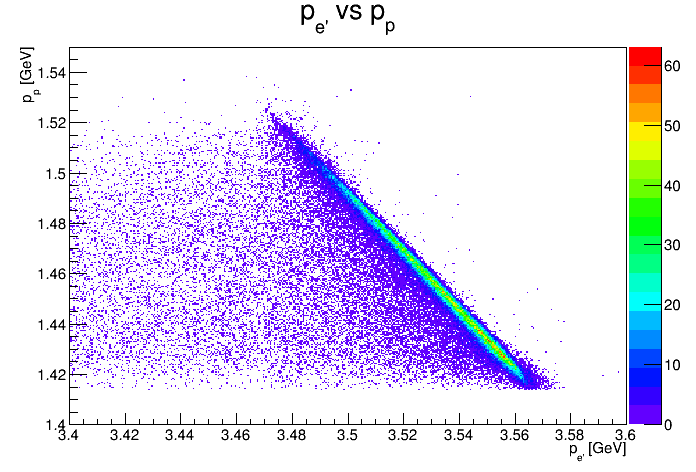
\includegraphics[width=15cm]{Pp_Pe.png}\\
Scattered electron and proton momentum.
\end{center}

\begin{center}
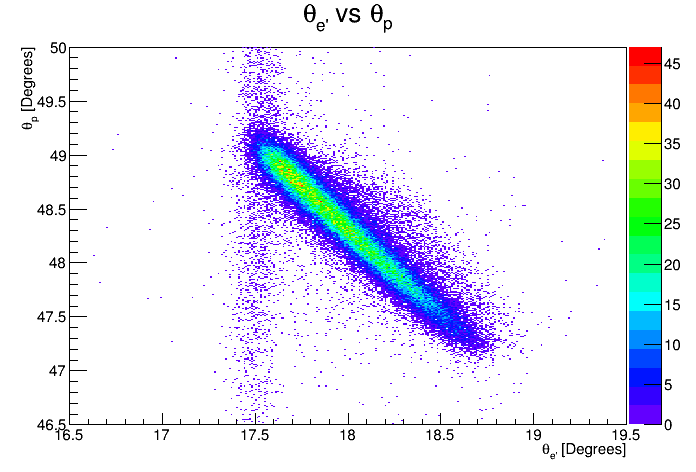
\includegraphics[width=15cm]{Tp_Te.png}\\
Scattered electron and proton angle.
\end{center}

\begin{center}
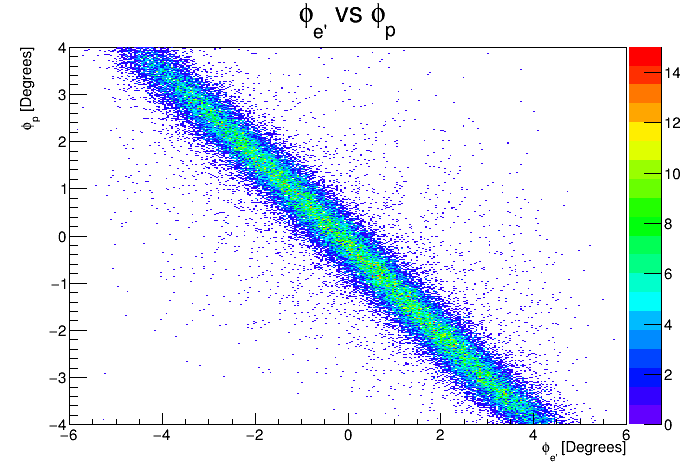
\includegraphics[width=15cm]{DelPhi.png}\\
Scattered electron and proton phi.
\end{center}

\clearpage
Now we can look at the difference in what is stored in the skimmed root tree, and what we can calculate/expect based solely on the scattering angles. This difference is shown in blue. \textbf{All variables called ``expected" refer to kinematics based on measured scattering angles}. Recall that the point is the two should agree, and if they do not, I correct the variables based on the overdetermined system. The red curve corresponds to what was previously reconstructed \textbf{before} the optimization procedure. The difference between the red and blue curves represent only the optimized calibration shifts in central angles/momenta.\\

\begin{center}
\includegraphics[width=13cm]{delE1.png}\\
Difference in calculated $E_1$ with measured beam energy, in GeV. The red curve is before corrected central angles of LHRS and RHRS.
\end{center}

\begin{center}
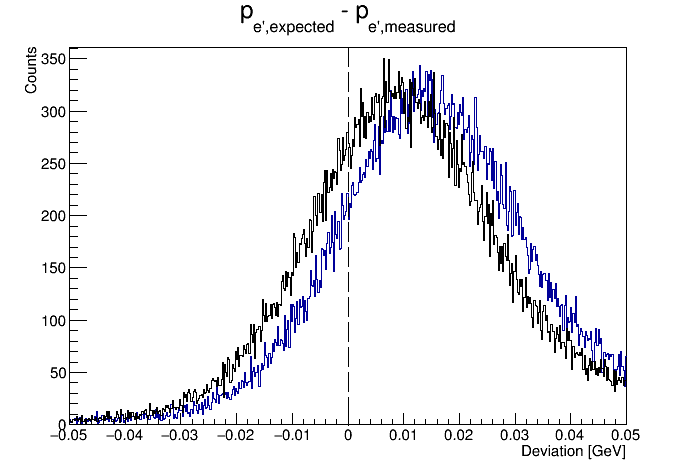
\includegraphics[width=13cm]{delPe.png}\\
Difference in calculated $E_3$ with what was measured by LHRS, in GeV. The red curve is before corrected central angles/momenta of LHRS and RHRS.
\end{center}

\begin{center}
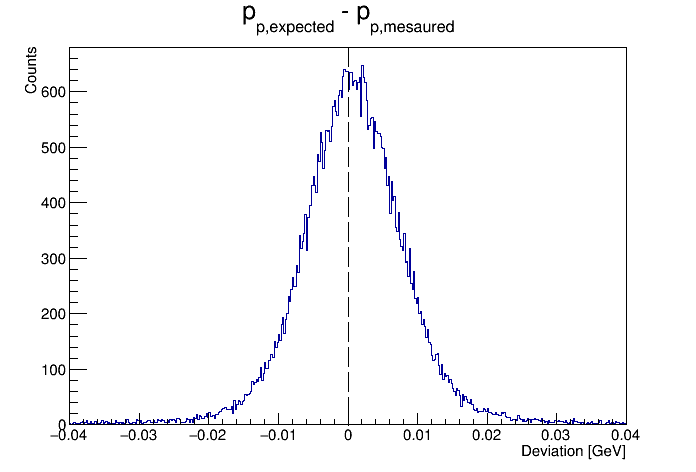
\includegraphics[width=14cm]{delPp.png}\\
Difference in calculated $\vec{p}_4$ with what was measured by RHRS, in GeV. The red curve is before corrected central angles/momenta of LHRS and RHRS.
\end{center}

\begin{center}
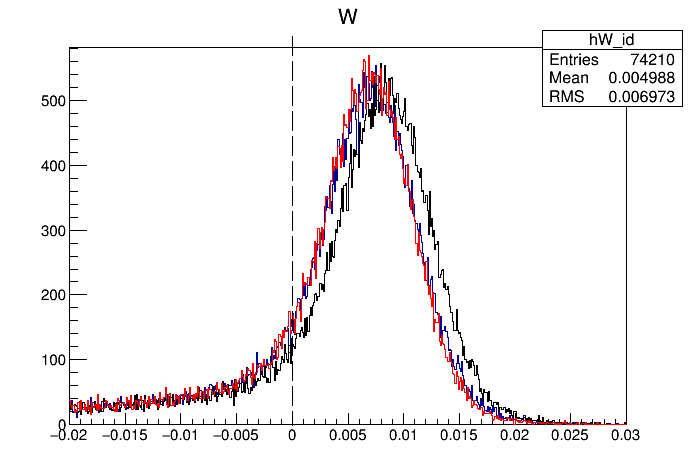
\includegraphics[width=14cm]{delW.png}\\
Difference with what was reconstructed based on measured quantites with $m_P$. The red curve is before corrected central angles/momenta of LHRS and RHRS.
\end{center}

\clearpage

And finally, measured missing momentum distributions before and after corrections. \textbf{These are reconstruced based on measured quantities, and should be 0 for $(e,e'p)$}
\begin{center}
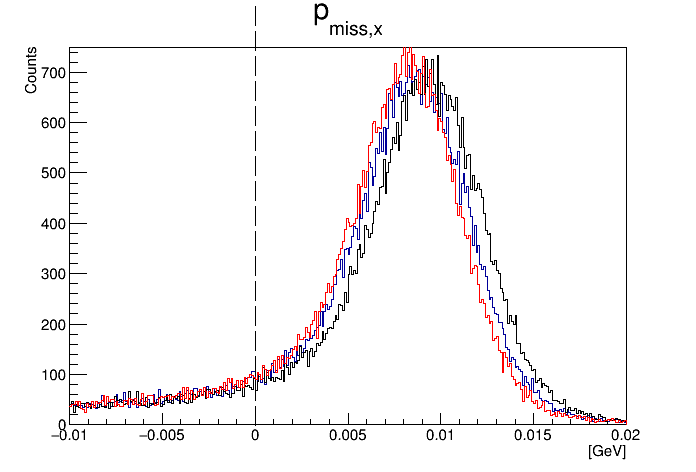
\includegraphics[width=14cm]{Pmx.png}\\
Measured $p_{\textrm{miss},x}$ distributon.
\end{center}

\begin{center}
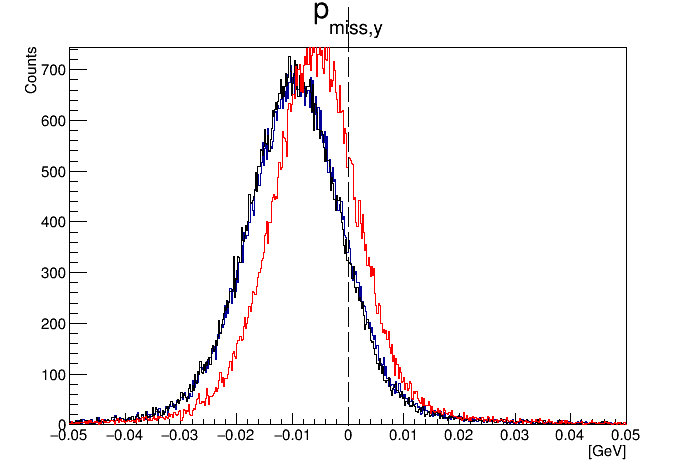
\includegraphics[width=14cm]{Pmy.png}\\
Measured $p_{\textrm{miss},y}$ distributon. Clearly this was not affected by any optimizations. The thought is that there is a more dominant source of error, likely the raster calibration is not optimized.
\end{center}

\begin{center}
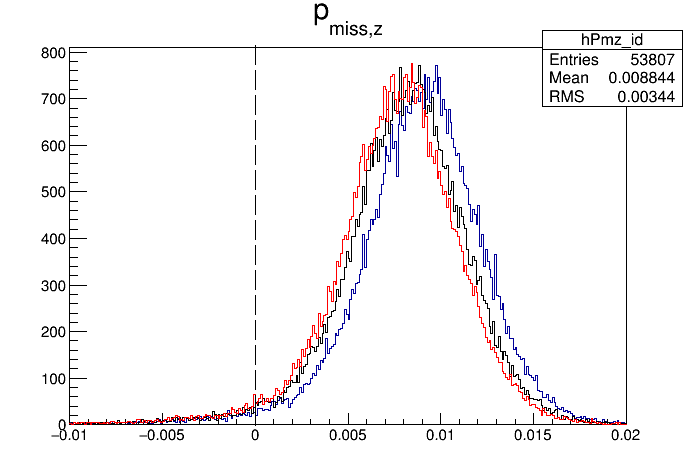
\includegraphics[width=14cm]{Pmz.png}\\
Measured $p_{\textrm{miss},z}$ distributon.
\end{center}

\begin{center}
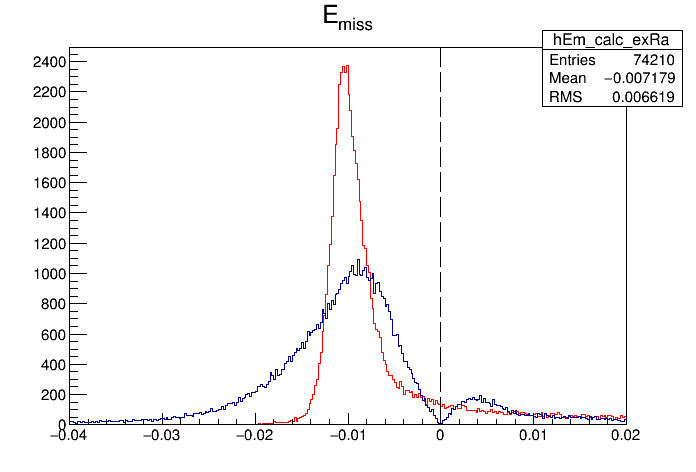
\includegraphics[width=14cm]{Em.png}\\
Measured $E_{\textrm{miss}}$ distributon.
\end{center}

\clearpage


%%%%%%%%%%%%%%%%%%%%%%%%%%%%%%%%%%%%%%%%%%%%%%%%%%%%%%%%%%%%%%%%%%%%%%%%%%%%%%%%%%%%%%%%%




\end{document}
